\chapter{Do interacting species co-occur differently from not-interacting species?}
\label{chap3}

\section{Résumé en français du troisième article}

Dans ce troisième article, je me suis me confronter aux données d'occurrence qui sont une données essentielle en biogéograhie pour répondre avec ces données à la question centrale de ma thèse~:Afin de répondre èà la quetsion centrale de ma thèse sur le rôle des interactions dans les conséquencens
Le but de l'article est de tester les prédictions du chapitre précédents, pour évaluer la pertinence d'utiliser l'information
contenue dans les réseaux écologiques pour expliquer les co-occurrences.
Bien que la théori ait été dévoloppé, les données requisent osnt particulièrement rares car elles demandesnt des distribution d'une même communauté sur un large gradient. Dominique Gravel a cependent réussi à réunir de tels jeux de données. Notamment grâce à la partcipiation de Thomas Roselin, Bo Dalsgaard, Wilfred Thuillier, Benjamin Baiser qui nous ont données accès à quatre jeux de données dont les efforts pour les constitués ont été conséquents et je suis redevable à tous ceux qui ont permis la réalisation.

J'ai anlyser la co-occurrence à la lumnière du réseaux pour certain jeux de donnes les inetraction spour un jeux de données sur les arbres nous avons sonctruit un arbre de trait fincitonnel et suput.é uteacrtion. Nos résulats jettent une lumière forteintéressante nous montrons que quand les espèces sont éloignos dans  que les inetractions ont très porbablement un effet sur la co-occureence mais que la détection de cet effet est très vite rendu impossible quand 1) les espèces sont éloignés dans le réseaux et 2) quand les interactions sont nombreuses. Les interaction indirectes n'ont donc pas d'effet mais aussi le nombre affecte notre capcité de sdetection. Il ne fat donc pas conslue et aussi pensé que ce qui est vrai dans un mondre riche en esèces ne l'est pas quand nous alterrons la biovidersité.



\subsection{Publication envisagée}

Due à la nouveauté de nos résultats et la qualité des données j'envsage, J,ai rédigé je serais premier auteur, Dominique Gravel à supervisé dernier et tous les auteures ayanit apportés des données et aprticipé à la rédaction serint includ dans la liste des auteurs. Nous souhaiterins publié dans un et nuso envsoageon de sounettre dans les prochaines semaines à \emph{Proceedings of the National Academy of Sciences} ou le récent journal \emph{Nature Ecology \& Evolution}.



\emph{Les sections qui suivent sont celles de l'article envisagé.}


\newpage
\section{Context}\label{context}

Biogeographers are still debating about whether the biotic interactions
at the local scale impact large scale species distribution. If this is
indeed the case, then we should expect pairs of species to exhibit
non-random distribution at the large spatial scale. The observation of
independent species occurrences would therefore support the use of
classical species distribution models (hereafter SDMs,
\citet{Elith2006}) and confirm scenarios that have been proposed over
the last decade \citep{Thuiller2005, Thuiller2011, Albouy2012}, whereas
the observation of occurrence clearly related to interactions would give
credit to methods interpreting co-occurrence as a proxy for ecological
interactions \citep{Morales-Castilla2015} and encourage the use of joint
species distribution models \citep[hereafter
JSDM,][]{Ovaskainen2010, Pollock2014}. In order to test whether
interactions influence species distributions, the simplest avenue is to
investigate species co-distribution in light of their ecological
relationships. Such investigations started with Diamond's original study
stating that species interacting by competition should avoid each other
in space, leading to a `checkerboard' distribution \citep{Diamond1975}.
This idea was rapidly criticized for the lack of an adequate null
hypothesis \citep{Connor1979, Gilpin1982} and has led to a major
controversy that has lasted more than 30 \citep{Connor2013} and has
underlined the need for null models in ecology
\citep{Connor1983, Gotelli2000}. Furthermore, the absence of adequate
datasets has long prevent to test adequately this hypothesis.

Species ranges are very often inferred from the realized distribution,
which results from the joint impacts of abiotic and biotic environmental
factors along with dispersal limitations and historical contingencies
\citep{Pulliam2000, Holt2009, Godsoe2010a, Araujo2014}. Finding evidence
of the effect of species interactions on distribution may prove
technically difficult as it requires to discriminate the fundamental
niche from co-occurrence data (Box 1), which could explain the scarcity
of studies reporting such effect \citep[but see][]{Gotelli2010}.
Fortunately, recent developments in co-occurrence theory promises novel
avenues in which highly dimensional species distribution data could be
analyzed, accounting for the structure of the network of ecological
interactions \citep{Cazelles2016}. It has notably been proposed that the
higher the degree of a species, \emph{i.e} the number of species which
with it interacts, the weaker will be the detection of a signal of
co-occurrence. The geographical range of a species is indeed partially
correlated with all the ranges of species it is linked to, which should
blur the signal the interactions leave on pairwise co-occurrence,
however, a signal may persist in the co-occurrence of the focal species
with the joint distribution of the species it interacts with is
considered.\\
Also, two co-occurring species may be part of the same ecological
network but separated by several interactions, for such case, it has
been suggested that the longer the shortest-path, \emph{i.e} the number
of links between two species, the smaller the signal of co-occurrence.
Hence, based on co-occurrence data and information pertaining to
ecological network, the hypotheses recently formulated on the signal of
co-occurrence can be tested (Box 1).

Despite the fantastic number of studies investigating co-occurrence in
order to understand community assembly, the hypothesis that species
interactions should result in non-random associations in space has never
been tested formally. It is rather implicitly assumed in every
investigation. Our objective in this study is therefore to test this at
the scale of species range. We analyzed species association within five
different datasets ranging from plant-seed dispersers, host-parasitoids,
microbes, birds and forest trees. We quantify co-occurrence and
conditional co-occurrence accounting for abiotic constrains for species
that are known to interact and known to not interact directly. This is
an unique opportunity to test the hypotheses recently developed. We
report some signal of positive co-occurrence among the datasets,
suggesting a difference between pairs of interacting species and pairs
of not-interacting. We also point out that the degree of a species in a
network influences our ability to detect significant associations.
Moreover, we discover a clear relationship between the strength of
species associations and the cumulated occupancy of the entire set of
species with which a species interact. However, all the signal we
detected are weakened or even disappear once abiotic similarities among
site are integrated. We further discuss the integration of biotic
interactions in distribution models in the light of our results.

\section{Material and Methods}\label{material-and-methods}

\subsection{Datasets}\label{datasets}

We analyzed five datasets spawning a large diversity of organisms and
types of interactions (see \citet{tbl:id}), across an extensive gradient
of environmental conditions (see Fig S1 and SI Text). Our criteria for
selecting datasets were as follow: i) the occurrence data must have been
collected at the local scale, it could not be derived from range maps;
ii) data included observed absences; iii) occurrence was observed for
all species, not only a singe layer; interactions were known a priori;
v) since we are computing co-occurrences, which is typically a fairly
rare event, we needed an elevated number of sampling units. Direct
interactions were documented for four datasets and represented by
networks of ecological interactions: the Willow Leaf Network (WLN), the
Pitcher Plants Network (PPN), the Caribbean Hummingbirds Network (CHN),
the French Breeding Birds Survey (FBBS). We derived metawebs for each
network, \emph{i.e}, the matrix recording all interactions, and computed
three metrics among species from a regional pool: the connectance of
metawebs (proportion of realized interactions), the degree of species
(number of links for one species) and the shortest-path between all
pairs of species (the minimum number of link from one species to the
other, see SI Text). For the North American Trees (NAT) dataset, we
approximated competitive interactions by computing functional distance
between every pair of species (see table S1 and Fig S2). A similar proxy
for ecological interactions was also computed for the FBBS see table
S2). Only species that were present at least on 1\% of the total number
of observations were considered for the analysis (see SI Text).

\subsection{Quantifying co-occurrence}\label{quantifying-co-occurrence}

For each pair of species \(i\) and \(j\), we computed the number of
observed co-occurrence \(O_{i,j}\) and the expected number of
co-occurrence under independent distribution \(E_{i,j}\) and the
standard deviation associated \(SD_{i,j}\). We report the Z-score
\(O_{i,j}-E_{i,j}/SD_{i,j}\) \citep{Gilpin1982}, a standardized metric
of co-occurrence, with positive (negative) values indicating more (less)
co-occurrence relative to the random expectation. Expectations were
derived using three different methods. First, we assumed that all sites
were equivalent, meaning we ignored the potential influence of abiotic
conditions across the entire range. The observed co-occurrence is an
estimate computed from a limited number of observations
\citep{Gilpin1982, Veech2013} and therefore, we also considered an
hypergeometric distribution, which corrects for limited sample size (see
SI Text for further details). We used two different SDMs in order to
account for the abiotic environment and correct the random expectations,
namely, Generalized Linear Model (hereafter GLM) and Random Forest
(hereafter RF - see SI Text for more details and Fig S3 for the
assessment of models' performances). The correction using SDMs accounts
for the fact that species may co-occur simply because they have similar
abiotic requirements, irrespective of if they interact or not.

\section{Results}\label{results}

Without accounting the abiotic context, we observe a difference in the
strength of spatial associations between interacting and not-interacting
species (\ref{fig:synth} panels A to D, white boxplots) for two out of
four datasets for which direct interactions were known. In all cases,
spatial associations were positive, indicating that interacting species
are co-occurring more often that randomly expected, irrespective of the
type of interaction. For the WLN, distinguishing herbivore-willow
interactions from herbivore-parasitoids revealed that the strength of
co-occurrence was stronger for the former than the latter ones
(\ref{fig:shtpth} A-B). Interestingly, we noticed that the higher the
mean degree of species in the dataset, the more difficult the detection
of a signal of interactions in co-occurrence was (\ref{fig:shtpth} A-D).

We observed that the strength of spatial association was higher for
pairs of similar species (\ref{fig:synth} panels E and F) for the NAT
and FBBS datasets, for which we inferred a distance based on functional
traits. Functional similarity is often interpreted as a proxy for
competition strength \citep{Morales-Castilla2015}, which according to
Diamond's hypothesis, should provide a negative association. However,
the observed associations are rather positive for functionally similar
species. This suggest that local competition is poorly detectable at
large scale which is theoretically supported \citep{Araujo2014} and the
positive associations are likely the results of similar physiological
requirements that cannot be taken into account given the sets of abiotic
variables we used. This is further supported by the regressions of the
Z-score against the distance (see Fig. S6 A-D). We also note that
results for the FBBS dataset were identical irrespective the type of
traits examined (Fig. S4). When we account for suitability discrepancies
among sites, \emph{i.e.} when we perform SDMs, the co-occurrence signals
we previously observed are weakened or disappeared. Co-occurrence
distributions are shifted toward 0 and dramatically shrunk (Fig.
\ref{fig:synth} panels A to D, grey and dark grey boxplots). The
tendencies are stronger for the RF approach than for the GLM one. The
same trends are observed when we used functional distance rather that
interactions (Fig. \ref{fig:synth} panels E-F).

We investigated if the strength of associations between species
interacting indirectly decreases with the shortest path (Fig.
\ref{fig:shtpth}). We examined the co-occurrence distribution against
the shortest-path for pairs of: herbivores and willows in WLN (A),
herbivores and parasitoids in WLN (B), hummingbirds and hosts plants (C)
and all pairs in PPN (D). Without accounting for the climatic factors,
we observe a decrease of the standardized co-occurrence with an
increased shortest-path for three out of four occurrence datasets (Fig.
\ref{fig:shtpth} A-D, white boxplots). This was predicted by the theory,
but the observed decay is steeper than anticipated \citep{Cazelles2016}.
We observed a similar but weaker decay when all pairs of species were
taken into account (see Fig. S5). Moreover, when we calculated the mean
degree in of predators (pollinators), we also found the signal of
co-occurrence stronger for specialists (Fig. \ref{fig:shtpth} A) than
for generalists (Fig. \ref{fig:shtpth} C), suggesting that the abundance
of interactions may prevent us from detecting them in static occurrence
data. Again, the tendencies observed are strongly weakened when
occurrence probability are derived from SDMs (Fig. \ref{fig:shtpth} A-D
grey and darker grey boxplots).

Finally, for all predators and pollinators in WLN, CHN and PPN, we
average the standardized co-occurrence over the set of their respective
preys (host plants) and plotted the obtained values against the total
number of site covered by the same set of preys (hosts) they refer to
(\ref{fig:degocc}). When abiotic context is not included, we observe a
clear negative relationship between the two quantities for three out of
four datasets. The associated linear regressions explain up to 69\% of
the variance (\ref{fig:degocc} panels A, D, G and J). However, the
linear regression poorly performed for the PPN, in which the connectance
is the highest. Additionally, we show that the linear regressions
outperformed the ones using the degree of the species (Fig S7 panels A,
D, G and J) that was envisioned by the theory \citep{Cazelles2016}.
Moreover, the relation is asymmetric: the decay is less convincing when
the the mean Z-scores of the preys are plotted against the cumulated
range of their predators (fig S8 panels A, D, G and J). These results
suggest that for a predator (pollinator) feeding upon a set of preys
(hosts), the detection of interactions is possible if the part of the
geographic range studied covered by the preys is low, when the part
increases our ability to detect the signal fades away. Once again, the
results are dramatically different once abiotic constrains were taken
into account: the clear relationship obtained is either weakened or even
reversed (\ref{fig:degocc} B,C,E,F,H,I,K,L). Even the strongest
associations seem to be captured by the SDMs, meaning they are captured
by the link with this environment but this questions how the inference
is made when the presence of one species is best explained by the
presence of its prey. Indeed, we show the presence of the whole set of
prey as predictor to assign the presence of specialist predator
outperform GLMs but not RFs (see Fig. S9).

\subsection{Discussion}\label{discussion}

The historical debate on co-occurrence triggered by Diamond's original
work was based on the idea that competitors must repulsed each other
\citep{Diamond1975}. Interestingly, we were not able to detect any
negative signal for species we assumed to compete. This support the idea
that local repulsion that must occur do not leave any mark on
co-occurrence data over a broad geographical gradient
\citep{Araujo2014}. However, we demonstrate that other signals, not
mentioned in the controversy, can actually be revealed. Mutualism and
predation were indeed detected as positive signals in the standardized
co-occurrence. Therefore, the interdependency between a predator
(pollinator) and its preys (host plant) makes them co-occurring more
than randomly expected and this effect is appreciable at large scale
\citep{Araujo2014}. Moreover, we find that the signal of co-occurrence
is blurred by the number of interactions a species experience, in
agreement with recent co-occurrence theory \citep{Cazelles2016}. As a
consequence, the distribution of a given species is more strongly
related to the distribution of the entire set of species it interacts
with, than each species taken individually. This indicates that the role
of ecological interactions may not only be a matter of spatial scale
\citep{McGill2010}, but also a matter of picking the most consistent
biological unit to investigate distribution over large spatial scales.

The signal of co-occurrence were dramatically reduced once we accounted
for the abiotic context. This could lead us to conclude that
co-occurrences are likely driven by the abiotic difference among site.
Climatic data doubtlessly explains a large part of the co-occurrence
observed, however our findings suggest a potential methodological issue.
Current SDMs always use abiotic constraints as the main drivers of
geographic distributions. In doing so, they capture, at least partially,
the impact of biotic interactions on distribution (as it infers the
distribution from the realized distribution). A predator is therefore
linked to its preys through the abiotic similarities of the sites where
they are found. However, the strength of an association may not be
perfectly captured by SDMs, this would explain why the relationship
vanishes in \ref{fig:degocc} when we used SDMs approach to derive
co-occurrence probabilities while the co-occurrence signal remains
positive. Understanding which part of the interactions is captured by
the SDMs remains of central important to build better distribution
models.

SDMs are based on the assumption that species are distributed
independently from each other and that scenarios of tomorrow's
biodiversity can be anticipated using abiotic variables only
\citep{Jeschke2008}. Some recent developments in statistics relaxed this
hypothesis by representing the distribution of assemblages, based on
correlations between species \citep{Pollock2014, Warton2015b}. The
development of these powerful statistical tools is essential, however it
can only provide a partial solution to some limitations of SDMs.\\
A substantial part of the solution lies in the understanding of the role
of ecological and evolutionary mechanisms shaping distributions
\citep{Thuiller2013}. Here, we underline the need for not hypothesizing
\emph{a priori} the independence among species. Rather, the assumption
must be proved to apply, otherwise a relevant assemblage must be
modeled. We suggest that for generalist species, the assumption of
independence is reasonable while for specialists the relative position
with the other species within the network should help deciding which set
of species are to be modeled. We therefore suggest that ecological
interactions should be integrated as prior information in SDMs to
strengthen our predictions. For instance, the range of a predator is
bounded by the range of the set of its preys
\citep{Holt2009, Shenbrot2007}, this reality should be integrated into
account when we predict the distribution of food webs, and predators'
ranges must be computed consistently with the predicted ranges of their
prey.

Our results lead us to conclude that co-occurrence tends to the
independence with increasing diversity of interactions. Only the
specialized species are strongly associated with their partners, as
generalists experience a much more diffuse constraint from interacting
species. Similarly, it it has been recently highlighted that net species
interaction strength better pairs of species is better predicted when
the species richness increases \citep{Berlow2009}. Further, press
perturbations applied to specialist species do have much stronger
indirect impacts on the other species than perturbations applied to
generalists \citep{Montoya2009}. All of these results are congruent with
MacArthur's vision, who more than 40 years ago, noticed the following
paradox \emph{``How can a more complex community be easier to
understand? A possible answer might be that the complex community have
strong interactions among species so that the lives of the separate
species are less independent than in a simple community. Where there is
greater interdependence, patterns may be more conspicuous.''}
\citep[p.199]{macarthur1972geographical}. In the present study, the more
the interactions among species the easier the forecasting of species
distribution. However, under the ongoing mass extinction, a myriad of
links vanishes while new ones emerge with the changes in the composition
of local communities. Therefore, even if under current conditions the
assumption of independence may be valid, under dramatic modifications of
ecosystem as currently observed, it may often prove false. As a step
forward, new biodiversity scenarios must not solely map the future
ranges of individual species but the entire community including the
consequences of potential extinction on community structure.

\newpage

\subsection{Box 1}\label{box-1}

The fundamental niche is here defined as the occurrence probability
under the assumptions that (1) biotic factors are not limiting the
occupancy and (2) the occupancy is estimated in the absence of
immigration \citep{Godsoe2010a}. In this case, only abiotic factors
(such as water availability, temperature variability or edaphic
variables) limit survival and/or reproduction success, and then the
occurrence probability. For a four species network made of three trophic
levels: two primary producers, a predator feeding upon them and a top
predator, we first consider the fundamental niches \(f_i\)
(\ref{fig:box1} A). For the top predator, we derive the fundamental
niche under the assumption of the presence of its prey:

\[f_4(w)=P(X_4=1|X_3=1, G=w)\]

where \(G\) denotes the environmental gradient and \(X_i\) represents
the random variable of the presence of species \(i\). For the lower
predator, we consider its preys substitutable and we assume the presence
of at least one prey to allow the predator to be present:

\[f_3(w)=P(X_3=1|X_2+X_1>0, G=w)\]

Similarly, \(f_1\) and \(f_2\) are obtained assuming that 3 is absent:

\[f_2(w)=P(X_2=1|X_3=0, G=w)\]

and:

\[f_1(w)=P(X_1=1|X_3=0, G=w)\]

Once projected on a map, the fundamental niche unravels the potential
distribution of a species \citep{Kearney2004}. The expected distribution
can be compared to real observations and could reveal whether dispersal
limits and ecological interactions are prevalent in the occupancy
dynamics of studied species. The realized niche (\ref{fig:box1} B)
includes these factors.\\
In our simplified example, fundamental and realized niches of preys are
identical. The realized niche of the top predator is constrained by the
one of predator 3, \(r_3\), which it-self is constrained by the joint
realized niches of its preys:

\[r_3(w)=P(X_3=1|X_2+X_1>0, G=w)P(X_2+X_1>0, G=w)\]
\[r_3(w)=f_3(w)\left(1-(1-r_1(w))(1-r_2(w))\right)\]

Then, assuming that species 4 do not alter \(r_3\), we have:

\[r_4(w)=f_4(w)r_3(w)\]
\[r_4(w)=f_4(w)f_3(w)\left(1-(1-r_1(w))(1-r_2(w))\right)\]

The above expressions may often be more complicated due to immigration
fluxes as well as the size and the structure of the interaction network.
For instance, we do not consider the apparent competition between
species 1 and 2, although it must affect their co-distribution.
Integrating the impact of many interactions may be possible using
occurrence probabilities of species assemblages rather than single
species \citep{Cazelles2016}. Here, the realized niches of predators 3
and 4 depends on the fundamental niches of preys 1 and 2.

The link between the fundamental niche and the distribution goes through
different ecological processes such as immigration and ecological
interaction \citep{Pulliam2000, Godsoe2010a}. The distribution we infer
is based on realized niche that includes the effect of abiotic variables
and biotic interactions. If we now examine the co-occurrence signals,
\emph{i.e.} the difference between the expected co-occurrence and the
observed co-occurrence \citep{Cazelles2016}, in empirical data, in order
to ascribe a particular signal to an ecological interaction, five
difficulties emerge:

\begin{enumerate}
\def\labelenumi{\arabic{enumi}.}
\tightlist
\item
  the signal of co-occurrence is not constant along the environmental
  gradient (\ref{fig:box1} C-a),
\item
  for species experiencing several interactions, the association with a
  particular species may be detectable only for a portion of the
  environmental gradient (\ref{fig:box1} C-b)
\item
  for species experiencing several interactions, the signal of
  co-occurrence with the set of species it interacts with might be more
  informative (\ref{fig:box1} C-c),
\item
  for species experiencing several interactions, the increase of
  interaction weakens the signal (this explain the drop for medium
  environmental values in \ref{fig:box1} C-c),
\item
  when the shortest-path between two species increase, the signal
  decreases (the red lines in \ref{fig:box1} C-c) is below the grey
  one).
\end{enumerate}

Using datasets including occurrence data for a large number of species
together with information pertaining to the ecological relationships, we
propose to test these theoretical expectations.

\newpage

\subsection{Tables}\label{tables}

\begin{longtable}[]{@{}lrrrrrrr@{}}
\caption{Data sets analyzed in this article.
\label{tbl:data}}\tabularnewline
\toprule
\begin{minipage}[b]{0.15\columnwidth}\raggedright\strut
Type\strut
\end{minipage} & \begin{minipage}[b]{0.07\columnwidth}\raggedleft\strut
No. of sites\strut
\end{minipage} & \begin{minipage}[b]{0.07\columnwidth}\raggedleft\strut
No. of species\strut
\end{minipage} & \begin{minipage}[b]{0.11\columnwidth}\raggedleft\strut
Interaction type\strut
\end{minipage} & \begin{minipage}[b]{0.05\columnwidth}\raggedleft\strut
Observed\strut
\end{minipage} & \begin{minipage}[b]{0.04\columnwidth}\raggedleft\strut
Traits\strut
\end{minipage} & \begin{minipage}[b]{0.06\columnwidth}\raggedleft\strut
Connectance\strut
\end{minipage} & \begin{minipage}[b]{0.22\columnwidth}\raggedleft\strut
References\strut
\end{minipage}\tabularnewline
\midrule
\endfirsthead
\toprule
\begin{minipage}[b]{0.15\columnwidth}\raggedright\strut
Type\strut
\end{minipage} & \begin{minipage}[b]{0.07\columnwidth}\raggedleft\strut
No. of sites\strut
\end{minipage} & \begin{minipage}[b]{0.07\columnwidth}\raggedleft\strut
No. of species\strut
\end{minipage} & \begin{minipage}[b]{0.11\columnwidth}\raggedleft\strut
Interaction type\strut
\end{minipage} & \begin{minipage}[b]{0.05\columnwidth}\raggedleft\strut
Observed\strut
\end{minipage} & \begin{minipage}[b]{0.04\columnwidth}\raggedleft\strut
Traits\strut
\end{minipage} & \begin{minipage}[b]{0.06\columnwidth}\raggedleft\strut
Connectance\strut
\end{minipage} & \begin{minipage}[b]{0.22\columnwidth}\raggedleft\strut
References\strut
\end{minipage}\tabularnewline
\midrule
\endhead
\begin{minipage}[t]{0.15\columnwidth}\raggedright\strut
Willow Leaf Network\strut
\end{minipage} & \begin{minipage}[t]{0.07\columnwidth}\raggedleft\strut
374\strut
\end{minipage} & \begin{minipage}[t]{0.07\columnwidth}\raggedleft\strut
156\strut
\end{minipage} & \begin{minipage}[t]{0.11\columnwidth}\raggedleft\strut
Trophic / Parasitism\strut
\end{minipage} & \begin{minipage}[t]{0.05\columnwidth}\raggedleft\strut
yes\strut
\end{minipage} & \begin{minipage}[t]{0.04\columnwidth}\raggedleft\strut
no\strut
\end{minipage} & \begin{minipage}[t]{0.06\columnwidth}\raggedleft\strut
0.042\strut
\end{minipage} & \begin{minipage}[t]{0.22\columnwidth}\raggedleft\strut
unpublished\strut
\end{minipage}\tabularnewline
\begin{minipage}[t]{0.15\columnwidth}\raggedright\strut
Pitcher Plants Network\strut
\end{minipage} & \begin{minipage}[t]{0.07\columnwidth}\raggedleft\strut
39x20\strut
\end{minipage} & \begin{minipage}[t]{0.07\columnwidth}\raggedleft\strut
53\strut
\end{minipage} & \begin{minipage}[t]{0.11\columnwidth}\raggedleft\strut
Trophic\strut
\end{minipage} & \begin{minipage}[t]{0.05\columnwidth}\raggedleft\strut
yes\strut
\end{minipage} & \begin{minipage}[t]{0.04\columnwidth}\raggedleft\strut
no\strut
\end{minipage} & \begin{minipage}[t]{0.06\columnwidth}\raggedleft\strut
0.44\strut
\end{minipage} & \begin{minipage}[t]{0.22\columnwidth}\raggedleft\strut
\citet{Baiser_2011}\strut
\end{minipage}\tabularnewline
\begin{minipage}[t]{0.15\columnwidth}\raggedright\strut
Caribbean Hummingbirds Network\strut
\end{minipage} & \begin{minipage}[t]{0.07\columnwidth}\raggedleft\strut
32\strut
\end{minipage} & \begin{minipage}[t]{0.07\columnwidth}\raggedleft\strut
62\strut
\end{minipage} & \begin{minipage}[t]{0.11\columnwidth}\raggedleft\strut
Mutualist\strut
\end{minipage} & \begin{minipage}[t]{0.05\columnwidth}\raggedleft\strut
yes\strut
\end{minipage} & \begin{minipage}[t]{0.04\columnwidth}\raggedleft\strut
no\strut
\end{minipage} & \begin{minipage}[t]{0.06\columnwidth}\raggedleft\strut
0.011\strut
\end{minipage} & \begin{minipage}[t]{0.22\columnwidth}\raggedleft\strut
\citet{MartinGonzalez2015}, \citet{Sonne2016}, \citet{Lack1973}\strut
\end{minipage}\tabularnewline
\begin{minipage}[t]{0.15\columnwidth}\raggedright\strut
North American Trees\strut
\end{minipage} & \begin{minipage}[t]{0.07\columnwidth}\raggedleft\strut
128891\strut
\end{minipage} & \begin{minipage}[t]{0.07\columnwidth}\raggedleft\strut
31\strut
\end{minipage} & \begin{minipage}[t]{0.11\columnwidth}\raggedleft\strut
Competition\strut
\end{minipage} & \begin{minipage}[t]{0.05\columnwidth}\raggedleft\strut
yes\strut
\end{minipage} & \begin{minipage}[t]{0.04\columnwidth}\raggedleft\strut
no\strut
\end{minipage} & \begin{minipage}[t]{0.06\columnwidth}\raggedleft\strut
-\strut
\end{minipage} & \begin{minipage}[t]{0.22\columnwidth}\raggedleft\strut
unpublished\strut
\end{minipage}\tabularnewline
\begin{minipage}[t]{0.15\columnwidth}\raggedright\strut
French Breeding Birds Survey\strut
\end{minipage} & \begin{minipage}[t]{0.07\columnwidth}\raggedleft\strut
2354\strut
\end{minipage} & \begin{minipage}[t]{0.07\columnwidth}\raggedleft\strut
179\strut
\end{minipage} & \begin{minipage}[t]{0.11\columnwidth}\raggedleft\strut
Trophic\strut
\end{minipage} & \begin{minipage}[t]{0.05\columnwidth}\raggedleft\strut
yes\strut
\end{minipage} & \begin{minipage}[t]{0.04\columnwidth}\raggedleft\strut
no\strut
\end{minipage} & \begin{minipage}[t]{0.06\columnwidth}\raggedleft\strut
0.018\strut
\end{minipage} & \begin{minipage}[t]{0.22\columnwidth}\raggedleft\strut
\citet{Gauzere2015}\strut
\end{minipage}\tabularnewline
\bottomrule
\end{longtable}

\newpage

\section{Figures}\label{figures}

\begin{figure}[htbp]
\centering
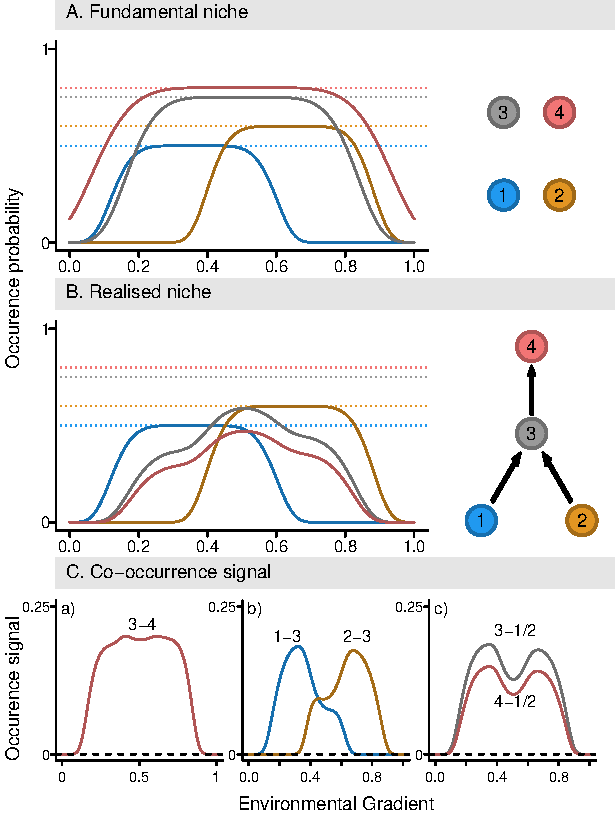
\includegraphics{chapitre3/figConcept.pdf}
\caption{\textbf{Probabilistic description of fundamental and realized
niches} For a four species network, all the occurrence probabilities are
derived along an environmental gradient assuming that (A) interactions
are not limiting the distribution and (B) that predators 3 and 4 needs
at least of one of its preys, \emph{i.e.} species 1 or 2. Horizontal
dotted lines in (A) and (B) stand for the occurrence probabilities
reached at an environmental optimum. The co-occurrence signal is
calculated for the following pairs : a) predators 3 and 4; b) predator 3
and prey 1, predator 3 and prey 1; c) predator 3 and prey 1 or 2,
predator 4 and prey 1 or 2. If no difference are found, 0 is
expected.\label{fig:box1}}
\end{figure}

\newpage

\begin{figure}[htbp]
\centering
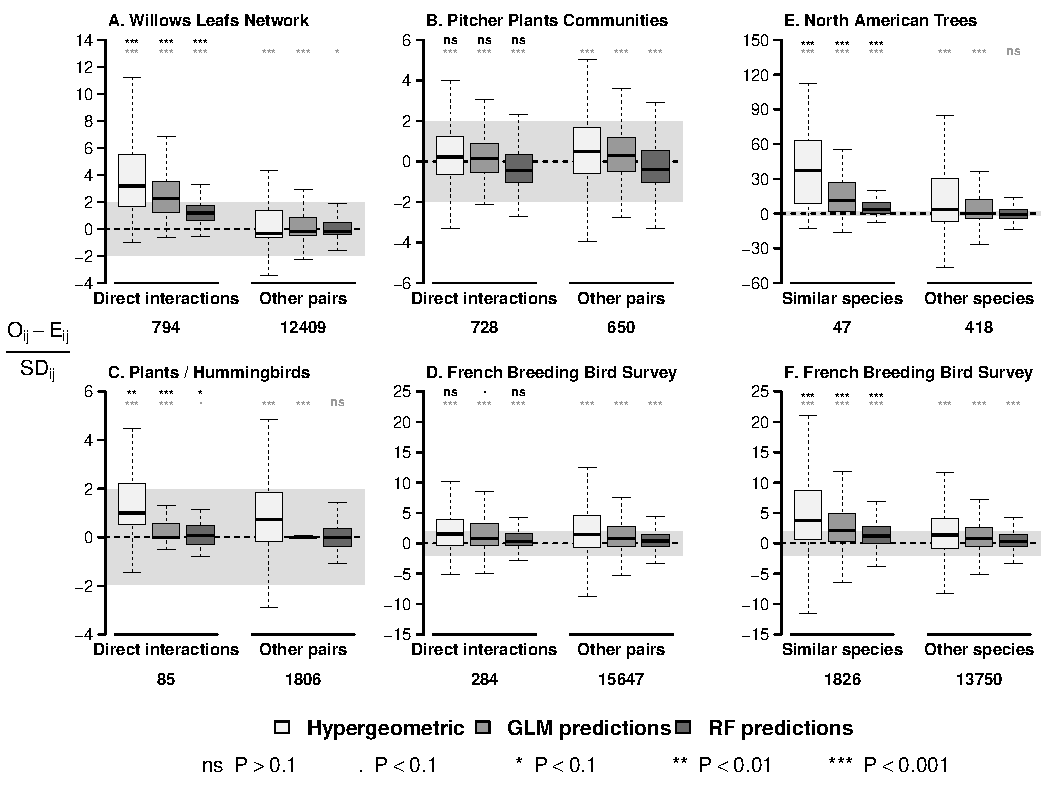
\includegraphics{chapitre3/figIntVsNoint.pdf}
\caption{\textbf{Co-occurrence of interacting versus not-interacting
pairs of species} Figures under each groups of boxplots indicate the
number of pairs to which the Z-score distributions refer. The light grey
rectangle corresponds to the 95\% confidence interval for the standard
normal distribution which gives insight into the proportion of pairs of
species significantly different from 0. The comparison made in panels A
to D is based on direct interactions observed. For panels E and F,
similar species are defined as the species for which the trait-based
distance is less than or equal to the lower decile of this distance
distribution. Note that outliers are not displayed. P values were
computed using the Wilcoxon rank sum test, to compare interacting versus
not-interacting Z-score distribution calculated for the three different
methods (black symbols) and to show whether the distribution is
symmetric about 0 (light grey symbols).\label{fig:synth}}
\end{figure}

\newpage

\begin{figure}[htbp]
\centering
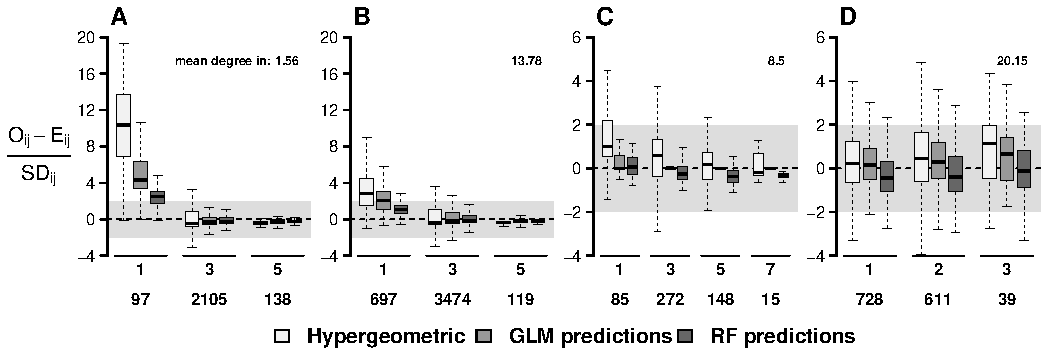
\includegraphics{chapitre3/figOrder.pdf}
\caption{\textbf{Co-occurrence signal decays when the shortest path
between a pair of species decay } The Z-score distribution are plotted
against the shortest path for A willows-herbivores interactions, B
herbivores-parasitoids interactions, C birds-plants interactions and D
the pitcher plants network. First figures under each grouped boxplots
indicate the shortest path associated while the figures below provide
the number of pair to which the distribution refers. Note that we used
the same y-axis for panels A and B as they regard two different kind of
interaction of the same dataset.\label{fig:shtpth}}
\end{figure}

\newpage

\begin{figure}[htbp]
\centering
\includegraphics{chapitre3/figdegocc.pdf}
\caption{\textbf{Co-occurrence significance decreases as the cumulated
occupancy increases} For a given species, Z-scores are averaged over the
all set species it interacts with and plotted against the joint
distribution of the same set of species. We do so for the herbivores in
the willows leafs network (panels A to C), the parasitoids in the willow
leafs network (panels D to F), the hummingbirds in the Caribbean
hummingbirds datasets (panels G to I) and all species in the pitcher
plants network that consume other species (panels J to L). The x-axis is
expressed as a log proportion of the total number of sites. Black
symbols are mean Z-scores significantly different from 0 (see SI Text).
In each panel, the dotted line represents the linear regression
\(y~ax+b\) for which the \(R^2\) is provided. The size of circles
reflects the degree of species for which the Z-score was calculated, the
relation size-degree for each row is given in the middle panel. For the
hummingbirds dataset (panels G to I), the triangle represent the values
obtained for the former distribution of a species already analyzed (see
SI text).\label{fig:degocc}}
\end{figure}

\newpage
\section{Material and methods}\label{material-and-methods}

In this section, we present in more details, the datasets and the
methodology we used. All analyses have been performed using R
environment software (table S1 includes functions and packages we used).

\subsection{Datasets}\label{datasets}

Sites for the five datasets are reported on five maps gathered in Fig
S1. The total number of species, the number of species present in at
least 1\% of the total number of site and the number of species for
which traits information were available are reported in table S2.

\paragraph{Traits-based distance}\label{traits-based-distance}

We used a distance built upon nine functional traits whose values were
retrieved from \citep{Paquette2011}, see \textbf{Supplementary Table 3}
available at
\url{http://onlinelibrary.wiley.com/doi/10.1111/j.1466-8238.2010.00592.x/suppinfo}.
Each of the nine selected variables were centered and scaled (R
functions used reported in table S1) then used as is to derive Euclidean
distances for all pairs of species. Then, we use agglomeration
clustering with Ward's method (implemented in the \emph{hclust()}
function we used, see Table S1) to obtain the dendrogram presented in
\ref{fig:dendro}.

\subsubsection{French Breeding Birds Survey
datasets}\label{french-breeding-birds-survey-datasets}

\paragraph{Traits-based distance}\label{traits-based-distance-1}

We used 73 traits that are boolean variable (see Table S4) we kept as is
to derive Euclidean distances for all pairs of species.

\subsection{Building metawebs}\label{building-metawebs}

For four datasets, we built network based on all observed interactions
and derived associated quantities, \emph{i.e.} the connectance of the
metawebs, the degrees of species and the shortest-path, using the R
package ``igraph'' (table S1).

\subsection{Co-occurrence measurement}\label{co-occurrence-measurement}

For a given pair of species \(i\) and \(j\), we examined the
relationship between the observed co-occurrence \(O_{i,j}\) and the
expected co-occurrence \(E_{i,j}\). Here, we provide more information
about the three methods wed used to analyse co-occurrence.

\subsection{Hypergeometric
distribution}\label{hypergeometric-distribution}

This distribution has been mentioned in a different context
\citep[see][]{Gilpin1982} and have been fully exploited in
\citet{Veech_2013} despite the author never mentioned it is a classical
distribution. To clarify this, we start from the distribution written in
equation (1) in \citet{Veech2013}. We consider the co-occurrence of two
species on \(n\) sites. Species 1 is present in \(n_1\) while species 2
is present in \(n_2\) sites. The probability of having \(j\)
co\_occurrence, \(p_j\) is:

\[ p_j= \frac{\binom{n}{j} \binom{n-j}{n_2-j} \binom{n-n_2}{n_1-j}}{\binom{n}{n_2} \binom{n}{n_2}} \]

if \(\max{0, n_1+n_2-n} \leq j \leq \min{n_1, n_2}\) and 0 otherwise.
The expression above yields:

\[ p_j= \frac{n!}{(n-j)!j!} \frac{(n-j)!}{(n-j-n_2+j)!(n_2-j)!} \frac{(n-n_2)!}{(n-n_2-n_1+j)!(n_1-j)!} \frac{(n-n_1)!n_1!}{n!} \frac{1}{\binom{n}{n_2}} \]

by rearrangement:

\[ p_j= \frac{1}{j!} \frac{1}{(n_2-j)!} \frac{1}{(n-n_2-n_1+j)!(n_1-j)!} \frac{(n-n_1)!n_1!}{1} \frac{1}{\binom{n}{n_2}} \]

once sorted out, this results in:

\[ p_j= \frac{\binom{n_1}{j} \binom{n-n_1}{n_2-j}}{\binom{n}{n_2}} \]

Thus, the number of co-occurrence follows a hypergeometric distribution
of parameters \((n,n_1,n_2)\) we used to calculated the expected
co-occurrence \(E_{i,j}\) under the hypothesis that all site were
identical for all species.

\subsection{GLM and RF}\label{glm-and-rf}

For GLM and RF, \(E_{i,j}\) correspond to probabilities of occurrence
computed based on climatic data. R functions are reported in Table S1.

\subsubsection{Climatic data}\label{climatic-data}

We used the global climate layers provided data WolrdClim, version 1.4,
available at \url{http://www.worldclim.org} \citep{Hijmans2005}. For
each dataset, we performed a principal component analysis and keep as
many axes as needed to explain 90\% of the total inertia. We used these
axis in GLM and RF.

\subsubsection{Generalized Linear Model}\label{generalized-linear-model}

For all datasets, we performed a Generalized Linear Model
\citep{Elith2006} using all the axis provided by the PCA as polynomials
of degree 2. To constraints the number of parameters, we did not
evaluate the interactions among axis. We also performed a selection
model based on the Akaike's information criterion (AIC) C in a Stepwise
Algorithm. R functions used to carry out the analyses are indexed in
table SX.

\subsubsection{Random Forests}\label{random-forests}

Random Forests \citep{Prasad2006} were performed using the same formula
as for GLMs. For all species, 10000 trees were computed and the
probability for a species being in a given site were calculated based on
the number of votes the sites were granted.

\subsubsection{Evaluating the models}\label{evaluating-the-models}

For all species, we assess the performance of the Species Distribution
Models we used, \emph{i.e.} Generalized Linear Model and Random Forest,
using the Area Under the Receiver Operating Characteristic (AUROC)
\citep{Elith2006}. We present the results as a cumulative sum of
frequencies corresponding to the score for all species for each of the
four ecological systems we studied (see Fig \citet{fig:idauc}).

\section{Supporting Tables}\label{supporting-tables}

\subsubsection{R packages used}\label{r-packages-used}

\begin{longtable}[]{@{}lrrrr@{}}
\toprule
Analysis & Function & Package name & Version & Citation\tabularnewline
\midrule
\endhead
Scaling and Centering & scale & base & 3.3.1 &
\citet{Rcoreteam2015}\tabularnewline
Euclidean distance & dist & stats & 3.3.1 &
\citet{Rcoreteam2015}\tabularnewline
Clustering & hclust & stats & 3.3.1 &
\citet{Rcoreteam2015}\tabularnewline
PCA & dudi.pca & ade4 & 1.7.4 & \citet{Dray2007}\tabularnewline
GLM & glm & stats & 3.3.1 & \citet{Rcoreteam2015}\tabularnewline
GLM Selection & step & stats & 3.3.1 &
\citet{Rcoreteam2015}\tabularnewline
Degree of species & degree & igraph & 1.0.1 &
\citet{Csardi2006}\tabularnewline
Shortest Paths & shortest.paths & igraph & 1.0.1 &
\citet{Csardi2006}\tabularnewline
AUROC & somers2 & Hmisc & 3.17.2 & \citet{Harrell2016}\tabularnewline
TSN retrieving & get\_tsn & taxize & 0.7.4 & \citet{hamberlain2013},
\citet{Chamberlain2016}\tabularnewline
Wilcoxon tests & wilcox.test & stats & 3.3.1 &
\citet{Rcoreteam2015}\tabularnewline
\bottomrule
\end{longtable}

\textbf{Supplementary Table 1}: R and packages used for the analyses.
GLM: Generalized Linear Model, PCA: Principal Component Analysis. AUROC:
Area Under the Receiver Operating Characteristic.\{\#tbl:code\}

\begin{longtable}[]{@{}lrrr@{}}
\toprule
Type & Total & Selected & Traits\tabularnewline
\midrule
\endhead
Willow Leaf Network & 274 & 156 & - ~\tabularnewline
Pitcher Plants Network & 91 & 53 & -\tabularnewline
Caribbean Hummingbirds Network & 62 & 62 & -\tabularnewline
North American Trees & 31 & 31 & 31\tabularnewline
French Breeding Birds Survey & 340 & 179 & 321\tabularnewline
\bottomrule
\end{longtable}

\textbf{Supplementary Table 2}: For each datasets the total number of
species (column \emph{Total}), the number of species present in more
that 1\% of the total number of sites (column \emph{Selected}), andthe
number of species for which traits information are available (column
\emph{Traits}). The symbol `-' means `not relevant'. \{\#tbl:numsp\}

\begin{longtable}[]{@{}lrrrrrrrrrr@{}}
\toprule
Species & TSN & maxH & GR & WD & TolS & TolD & AM & EM & LMA &
Nmass\tabularnewline
\midrule
\endhead
Abies balsamea & 18032 & 25 & 1 & 0.34 & 5.0 & 1.0 & 0 & 1 & 151.00 &
1.66\tabularnewline
Acer negundo & 28749 & 20 & 3 & 0.44 & 3.5 & 3.0 & 1 & 0 & 37.04 &
2.50\tabularnewline
Acer rubrum & 28728 & 25 & 3 & 0.49 & 3.4 & 1.8 & 1 & 0 & 71.09 &
1.91\tabularnewline
Acer saccharum & 28731 & 35 & 1 & 0.56 & 4.8 & 2.3 & 1 & 0 & 70.63 &
1.83\tabularnewline
Betula alleghaniensis & 19481 & 25 & 3 & 0.55 & 3.2 & 3.0 & 0 & 1 &
46.08 & 2.20\tabularnewline
Betula papyrifera & 19489 & 25 & 3 & 0.48 & 1.5 & 2.0 & 0 & 1 & 77.88 &
2.31\tabularnewline
Carpinus caroliniana & 19504 & 8 & 1 & 0.58 & 4.6 & 2.0 & 0 & 1 & 49.05
& 2.15\tabularnewline
Carya cordiformis & 19227 & 25 & 1 & 0.60 & 2.1 & 4.0 & 0 & 1 & 44.05 &
2.60\tabularnewline
Fagus grandifolia & 19462 & 25 & 1 & 0.56 & 4.8 & 1.5 & 0 & 1 & 61.22 &
2.04\tabularnewline
Fraxinus americana & 32931 & 30 & 2 & 0.55 & 2.5 & 2.4 & 1 & 0 & 76.75 &
2.12\tabularnewline
Fraxinus nigra & 32945 & 20 & 2 & 0.45 & 3.0 & 2.0 & 1 & 0 & 71.94 &
2.10\tabularnewline
Fraxinus pennsylvanica & 32929 & 25 & 3 & 0.53 & 3.1 & 3.9 & 1 & 0 &
87.72 & 1.80\tabularnewline
Larix laricina & 183412 & 25 & 3 & 0.48 & 1.0 & 2.0 & 0 & 1 & 120.00 &
1.36\tabularnewline
Ostrya virginiana & 19511 & 12 & 1 & 0.63 & 4.6 & 3.3 & 1 & 0 & 37.04 &
2.20\tabularnewline
Picea glauca & 183295 & 25 & 1 & 0.35 & 4.2 & 2.9 & 0 & 1 & 302.86 &
1.28\tabularnewline
Picea mariana & 183302 & 20 & 1 & 0.41 & 4.1 & 2.0 & 0 & 1 & 294.12 &
1.12\tabularnewline
Picea rubens & 18034 & 25 & 2 & 0.38 & 4.4 & 2.5 & 0 & 1 & 304.67 &
1.15\tabularnewline
Pinus banksiana & 183319 & 20 & 3 & 0.42 & 1.4 & 4.0 & 0 & 1 & 243.90 &
1.24\tabularnewline
Pinus resinosa & 183375 & 25 & 3 & 0.39 & 1.9 & 3.0 & 0 & 1 & 294.12 &
1.17\tabularnewline
Pinus strobus & 183385 & 30 & 3 & 0.36 & 3.2 & 2.3 & 0 & 1 & 121.92 &
1.42\tabularnewline
Populus balsamifera & 22453 & 25 & 3 & 0.37 & 1.3 & 1.8 & 1 & 1 & 83.46
& 1.95\tabularnewline
Populus grandidentata & 22463 & 20 & 3 & 0.39 & 1.2 & 2.5 & 1 & 1 &
70.45 & 2.50\tabularnewline
Populus tremuloides & 195773 & 25 & 3 & 0.37 & 1.2 & 1.8 & 1 & 1 & 82.02
& 2.16\tabularnewline
Prunus pensylvanica & 24799 & 12 & 3 & 0.36 & 1.0 & 2.0 & 1 & 1 & 50.00
& 2.40\tabularnewline
Quercus alba & 19290 & 35 & 1 & 0.60 & 2.9 & 3.6 & 0 & 1 & 81.21 &
2.39\tabularnewline
Quercus macrocarpa & 19287 & 15 & 1 & 0.58 & 2.7 & 3.9 & 0 & 1 & 92.74 &
2.27\tabularnewline
Quercus rubra & 19408 & 25 & 2 & 0.56 & 2.8 & 2.9 & 0 & 1 & 84.20 &
2.06\tabularnewline
Thuja occidentalis & 505490 & 15 & 1 & 0.30 & 3.5 & 2.7 & 1 & 0 & 223.00
& 1.02\tabularnewline
Tsuga canadensis & 183397 & 30 & 1 & 0.40 & 4.8 & 1.0 & 0 & 1 & 122.55 &
0.99\tabularnewline
Ulmus americana & 19049 & 35 & 3 & 0.46 & 3.1 & 2.9 & 1 & 0 & 79.47 &
2.07\tabularnewline
Ulmus rubra & 19050 & 25 & 3 & 0.48 & 3.3 & 3.0 & 1 & 0 & 59.88 &
2.50\tabularnewline
\bottomrule
\end{longtable}

\textbf{Supplementary Table 3}: Tree species and traits used.
Abbreviations are as follows: TSN - Taxonomic Serial Number defined by
Integrated Taxonomic Information System (ITIS), maxH - Average maximum
height, GR - Growth rate, WD - Wood Density, TolS - Shade tolerance,
TolD - Drought tolerance, AM - Arbuscular mycorrhiza (Endomycorrhiza),
EM - Ectomycorrhiza, LMA - Leaf mass per area, Nmass - Nitrogen content
per leaf mass unit\citep{Paquette2011} available at:
\url{http://onlinelibrary.wiley.com/doi/10.1111/j.1466-8238.2010.00592.x/suppinfo}.\{\#tbl:trees\}

\begin{longtable}[]{@{}lr@{}}
\toprule
Category & Trait name\tabularnewline
\midrule
\endhead
Activity & Nocturnal\tabularnewline
Activity & Crepuscular\tabularnewline
Activity & Diurnal\tabularnewline
Diet & Seeds, nuts or grain\tabularnewline
Diet & Fruits / frugivory\tabularnewline
Diet & Vegetative\tabularnewline
Diet & invert\tabularnewline
Diet & fish\tabularnewline
Diet & Very small mammals\tabularnewline
Diet & Large mammals\tabularnewline
Diet & Herptile\tabularnewline
Diet & Small birds\tabularnewline
Diet & Long birds\tabularnewline
Diet & Vertebrate\tabularnewline
Diet & Bones\tabularnewline
Diet & Carrion\tabularnewline
Feeding behavior & Pursuit (air and/or aquatic)\tabularnewline
Feeding behavior & Sally\tabularnewline
Feeding behavior & Foliage gleaning\tabularnewline
Feeding behavior & Pouncing\tabularnewline
Feeding behavior & Grazing\tabularnewline
Feeding behavior & Picking, pecking or stabbing\tabularnewline
Feeding behavior & Digging\tabularnewline
Feeding behavior & Overturning\tabularnewline
Feeding behavior & Probing\tabularnewline
Feeding behavior & Filtering\tabularnewline
Feeding habitat & Water-surface\tabularnewline
Feeding habitat & Underwater\tabularnewline
Feeding habitat & Water\tabularnewline
Feeding habitat & Mud\tabularnewline
Feeding habitat & Ground\tabularnewline
Feeding habitat & Canopy\tabularnewline
Feeding habitat & Shrub (low and high)\tabularnewline
Feeding habitat & Vegetation\tabularnewline
Feeding habitat & Air\tabularnewline
Foraging habitat & Wet grassland, meadows, fens, sedges or
tundra\tabularnewline
Foraging habitat & Dry grassland\tabularnewline
Foraging habitat & Rocky slope\tabularnewline
Foraging habitat & Fast river/stream\tabularnewline
Foraging habitat & Slow river/stream\tabularnewline
Foraging habitat & Shore (marine)\tabularnewline
Foraging habitat & Salt marsh\tabularnewline
Foraging habitat & Mud or silt\tabularnewline
Foraging habitat & Sandy gravel/beach\tabularnewline
Foraging habitat & Reed marshes\tabularnewline
Foraging habitat & Conifer\tabularnewline
Foraging habitat & Mixed forest\tabularnewline
Foraging habitat & Deciduous\tabularnewline
Foraging habitat & Mediterranean oak or other\tabularnewline
Foraging habitat & Open/low forest\tabularnewline
Foraging habitat & Forest or habitat edge\tabularnewline
Foraging habitat & Shrub/bush\tabularnewline
Foraging habitat & Urban\tabularnewline
Foraging habitat & Garden\tabularnewline
Foraging habitat & High air\tabularnewline
Nesting habitat & Wet grassland, meadows, fens, sedges or
tundra\tabularnewline
Nesting habitat & Dry grassland\tabularnewline
Nesting habitat & Banks/sand/mud\tabularnewline
Nesting habitat & Rock surface/outcrops\tabularnewline
Nesting habitat & Near water/shore/island\tabularnewline
Nesting habitat & Sand gravel/beach\tabularnewline
Nesting habitat & Reed marshes\tabularnewline
Nesting habitat & Conifer\tabularnewline
Nesting habitat & Mixed forest\tabularnewline
Nesting habitat & Deciduous\tabularnewline
Nesting habitat & Mediterranean oak and other\tabularnewline
Nesting habitat & Open/low forest\tabularnewline
Nesting habitat & Shrub/bush\tabularnewline
Nesting habitat & Urban\tabularnewline
Nesting habitat & Garden\tabularnewline
Nesting location & Elevated\tabularnewline
Nesting location & Tree hole\tabularnewline
Nesting location & Ground\tabularnewline
\bottomrule
\end{longtable}

\textbf{Supplementary Table 4}: List of the Boolean traits used to
derive Euclidean distances between all pairs of species in the French
Breeding Birds Survey.

\newpage

\section{Supporting Figures}\label{supporting-figures}

\begin{figure}[htbp]
\centering
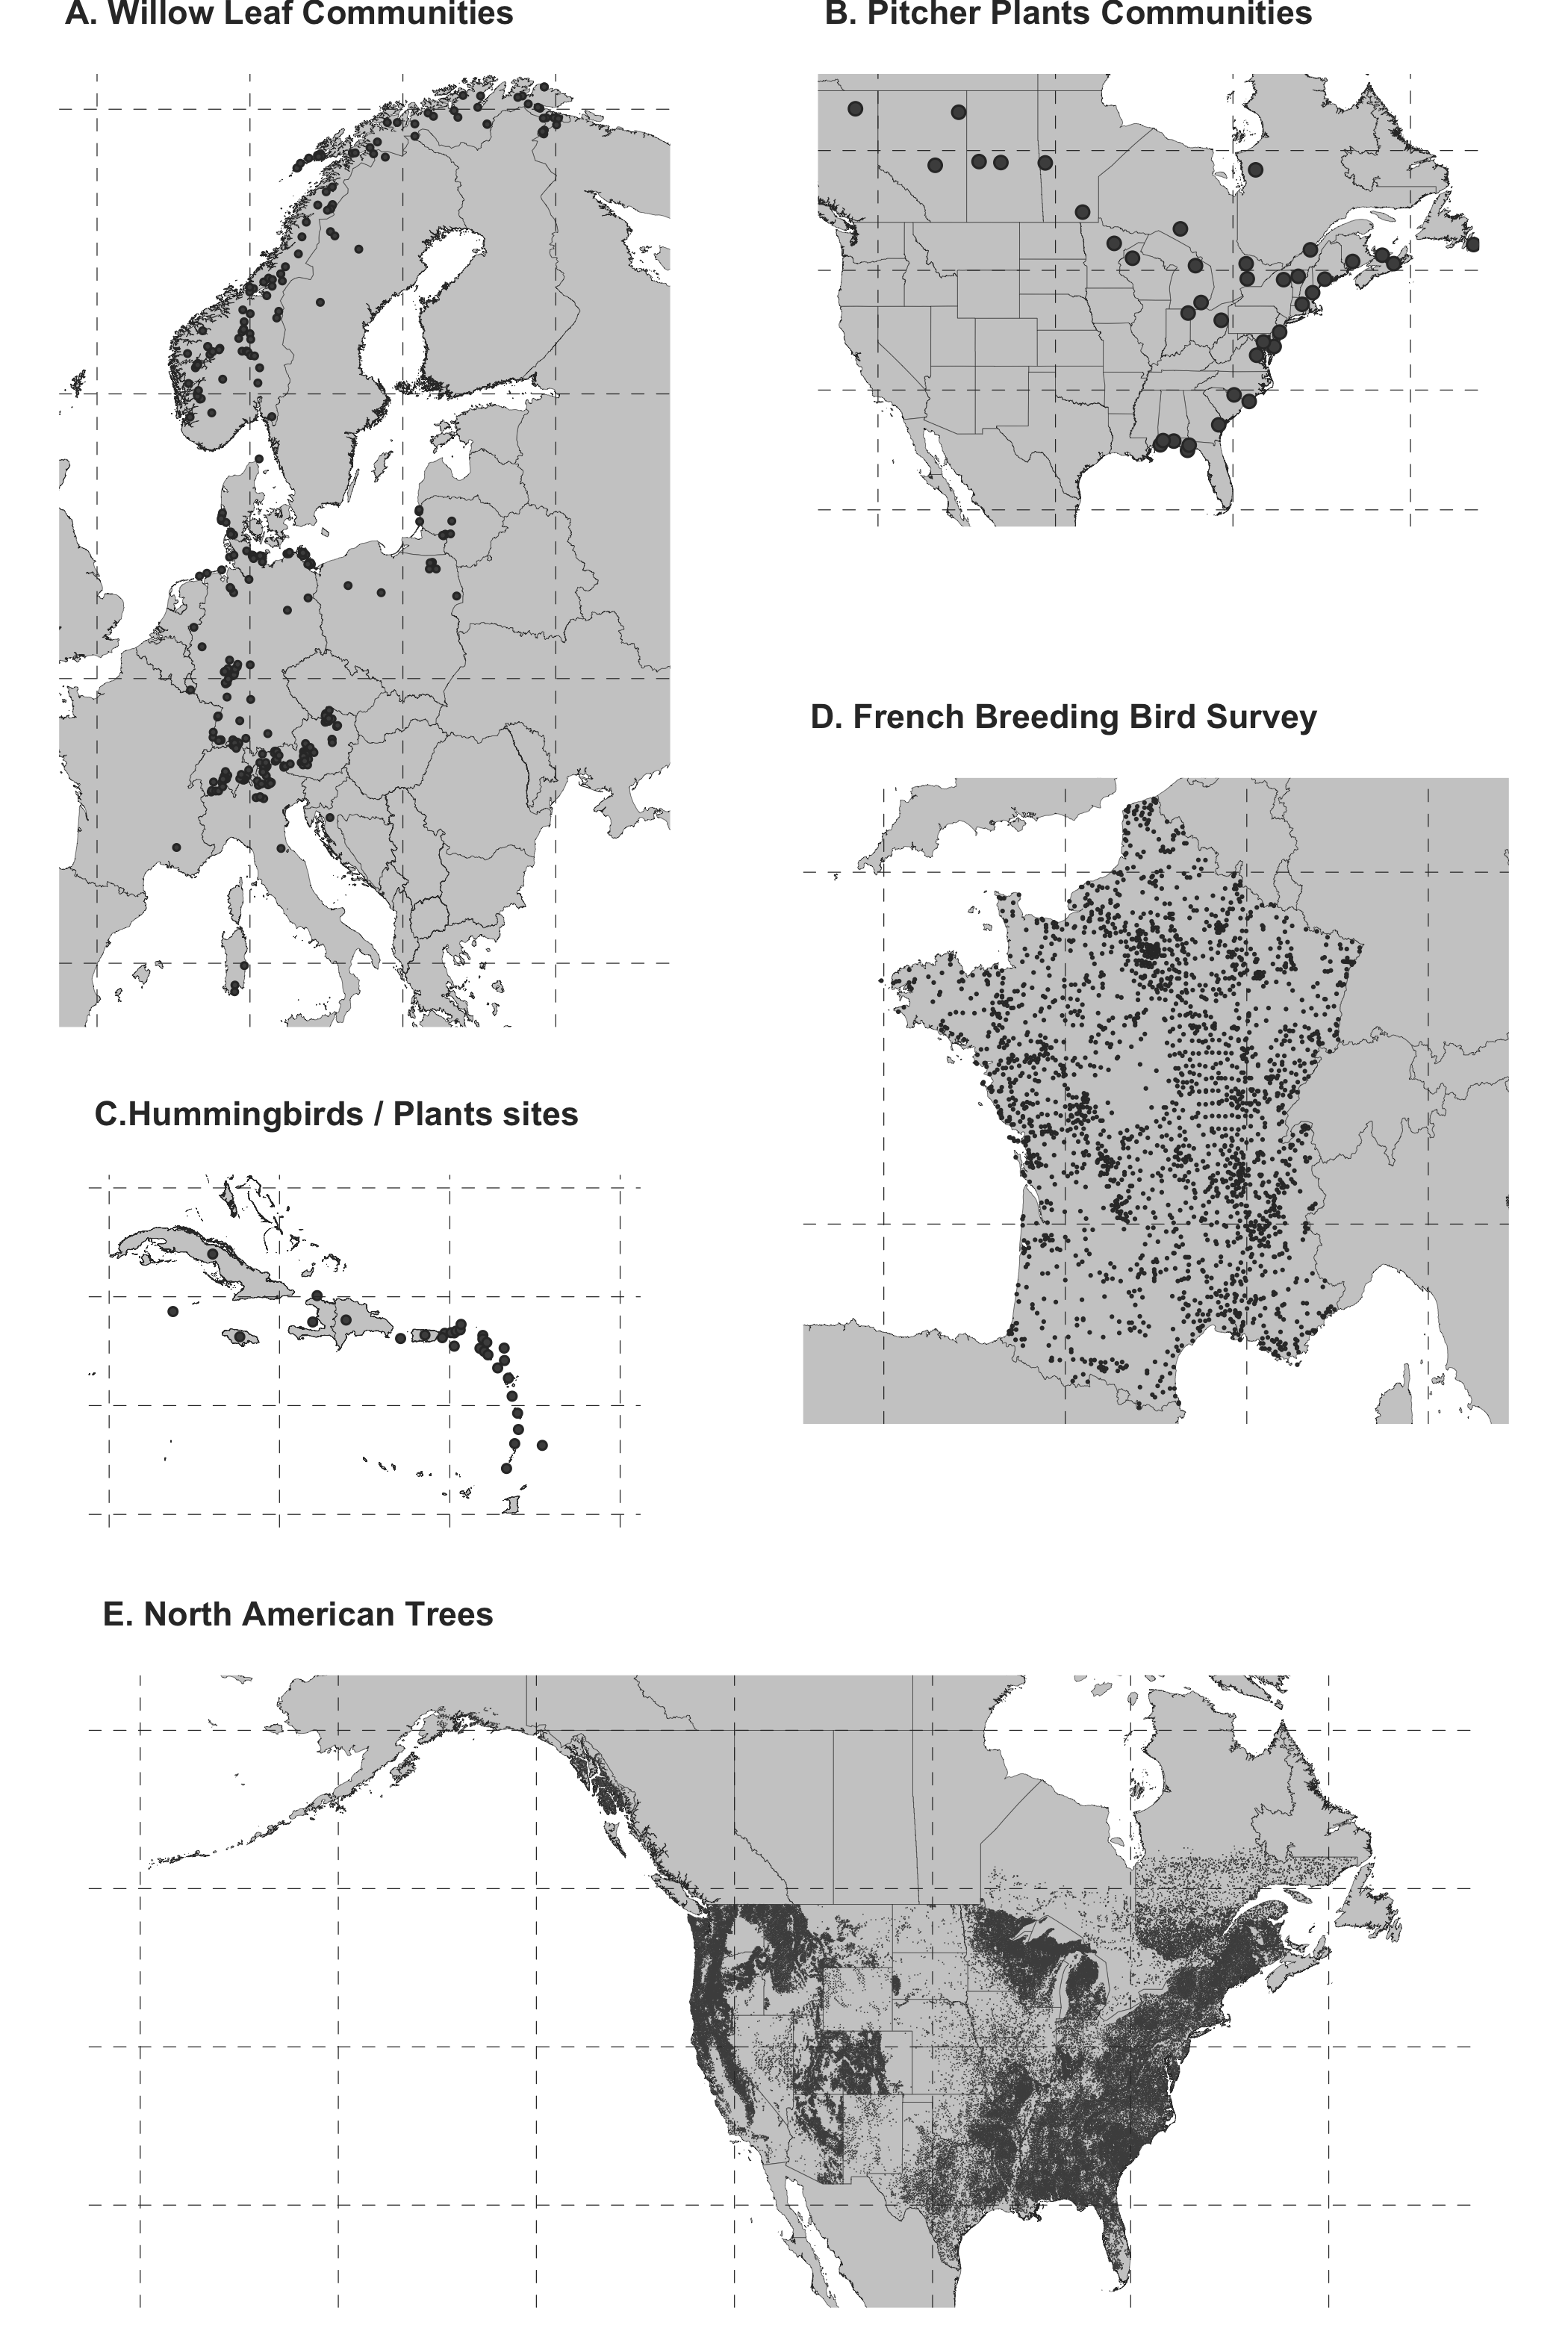
\includegraphics{chapitre3/figS1.png}
\caption{\textbf{Sites of the study}\label{fig:maps}}
\end{figure}

\newpage

\begin{figure}[htbp]
\centering
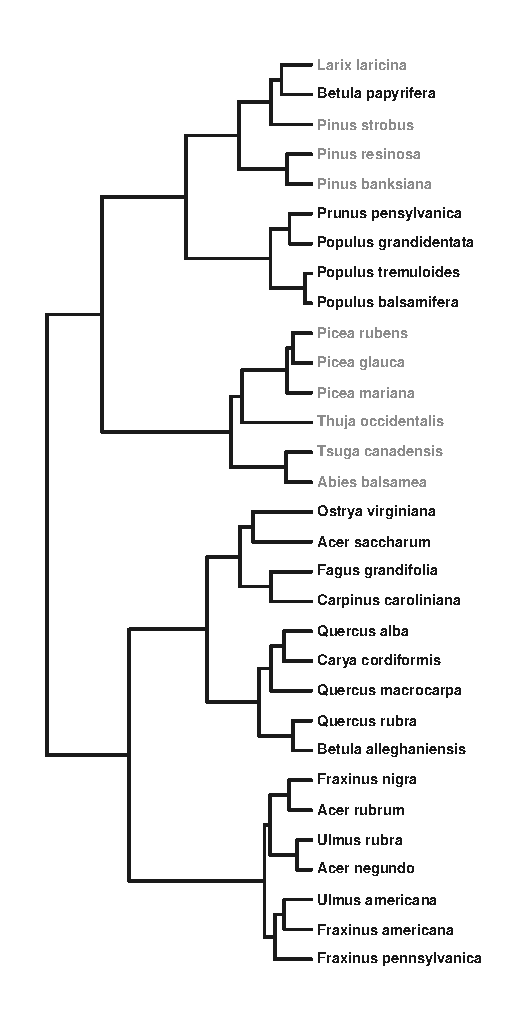
\includegraphics{chapitre3/figS2.pdf}
\caption{\textbf{Dendrogram representing the trait-based distances
between the 31 species studied in the North American tree datasets.}
Names of angiosperm species are written in dark grey while names of
Gymnosperm species are in a lighter grey.\label{fig:dendro}}
\end{figure}

\newpage

\begin{figure}[htbp]
\centering
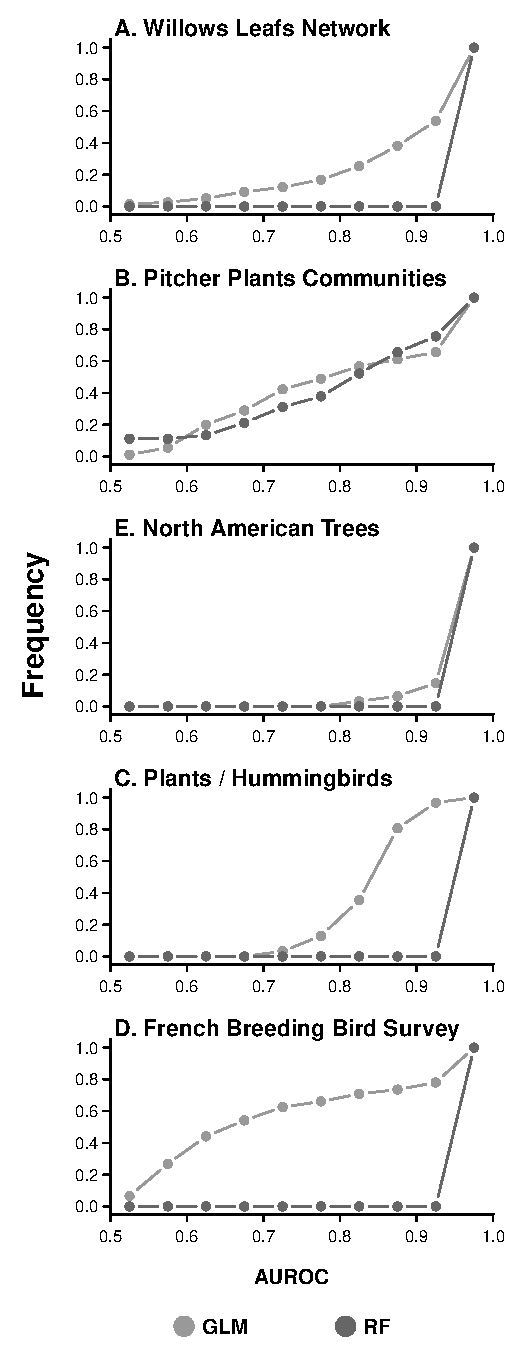
\includegraphics{chapitre3/figS3.pdf}
\caption{\textbf{Evaluation of the SDM approaches} For each dataset, the
distributions of performance of generalized linear models (light grey
symbols) and random Forest (dark grey symbols) for all species are
presented.\label{fig:auc}}
\end{figure}

\newpage

\begin{figure}[htbp]
\centering
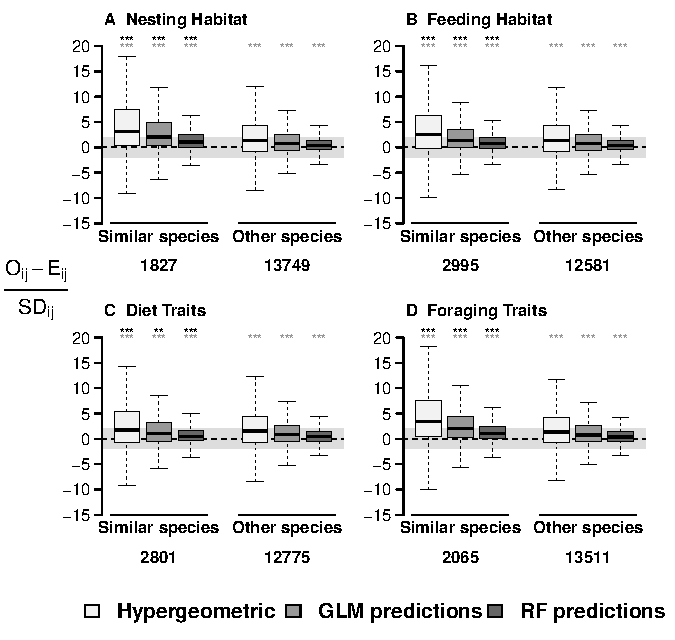
\includegraphics{chapitre3/figS4.pdf}
\caption{** Co-occurrence and the nature of the trait-based distance in
the FBBS dataset** The different panels correspond to four different set
of trait upon which for different distance are built. Similar species
are defined as the species for which the trait-based distance is less
than or equal to the lower decile of this distance distribution. Note
that outliers are not displayed. The light grey rectangle corresponds to
the 95\% confidence interval for the standard normal distribution which
gives insight into the proportion of pairs of species significantly
different from 0. P values were computed using the Wilcoxon rank sum
test, to compare interacting versus not-interacting Z-score distribution
calculated for the three different methods (black symbols) and to show
whether whether Z-score were greater for hypergeometric versus GLM and
whether GLM versus RF (grey symbols).}\label{figdist}
\end{figure}

\newpage

\begin{figure}[htbp]
\centering
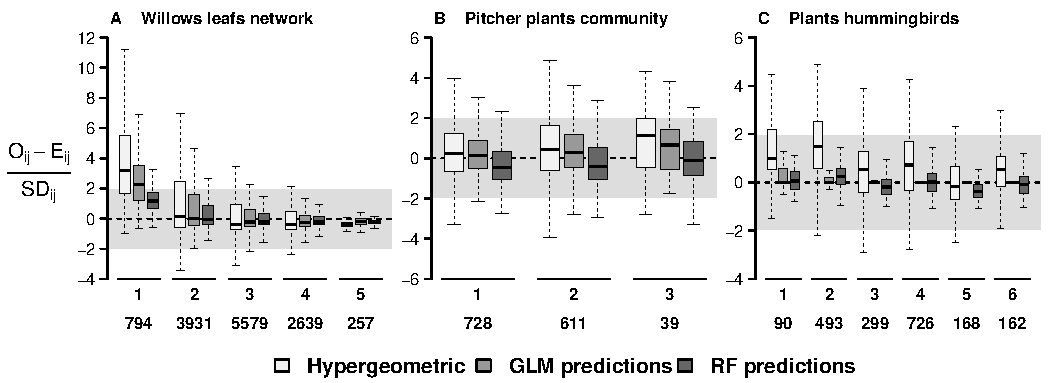
\includegraphics{chapitre3/figS5.pdf}
\caption{\textbf{Co-occurrence signal decays when the shortest path
between a pair of species decay} Distribution of Z-scores for all
interactions are grouped by shortest-path indicated by the first numbers
below boxplots. The other figures below stand for the number of pairs of
species included within the distributions.\label{fig:sht_pth2}}
\end{figure}

\newpage

\begin{figure}[htbp]
\centering
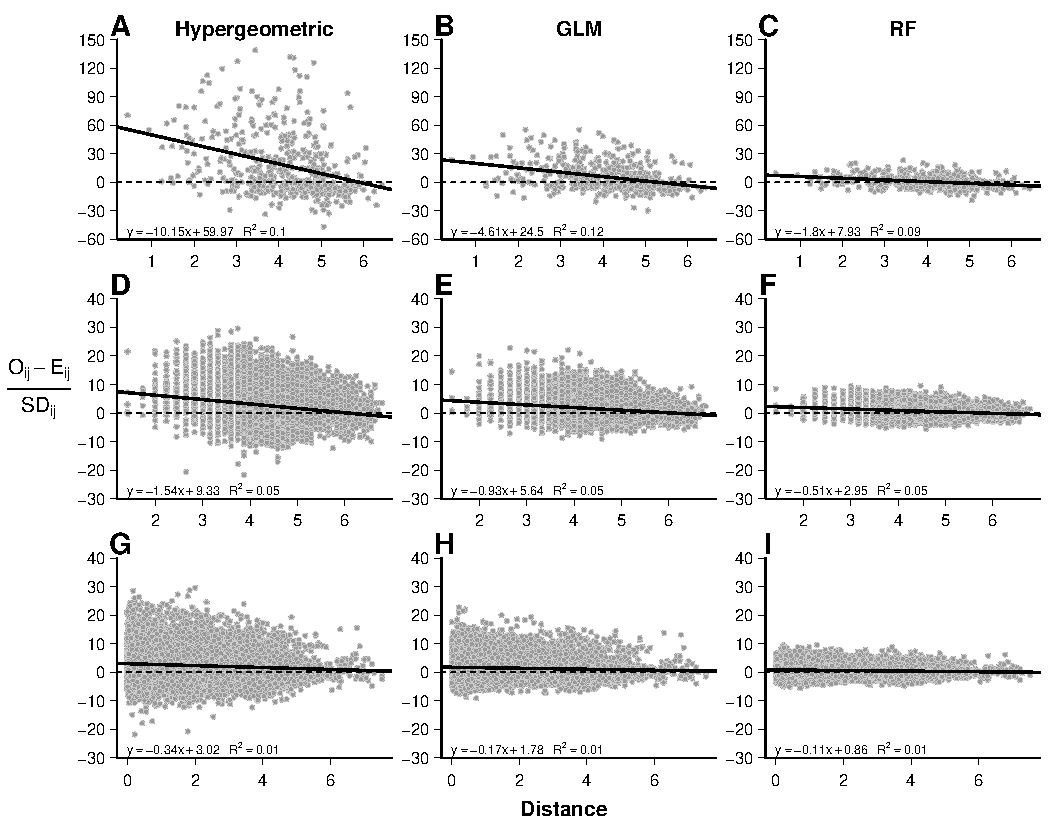
\includegraphics{chapitre3/figS6.pdf}
\caption{\emph{Changes co-occurrence signal when increasing the distance
between two species} Points represent the result for all pairs of
interaction for two datasets: the North American Tree dataset (A=C) and
the FBBS (D-I). For the latter, we used the trait-based distance
computed with all available traits (D-F) and the body-size ratios (the
lighter species over the heavier, panels G-I). In each panel, the
equation on the bottom-left corner indicated the results of the linear
regression depicted by the dotted line.\label{fig:distrev}}
\end{figure}

\newpage

\begin{figure}[htbp]
\centering
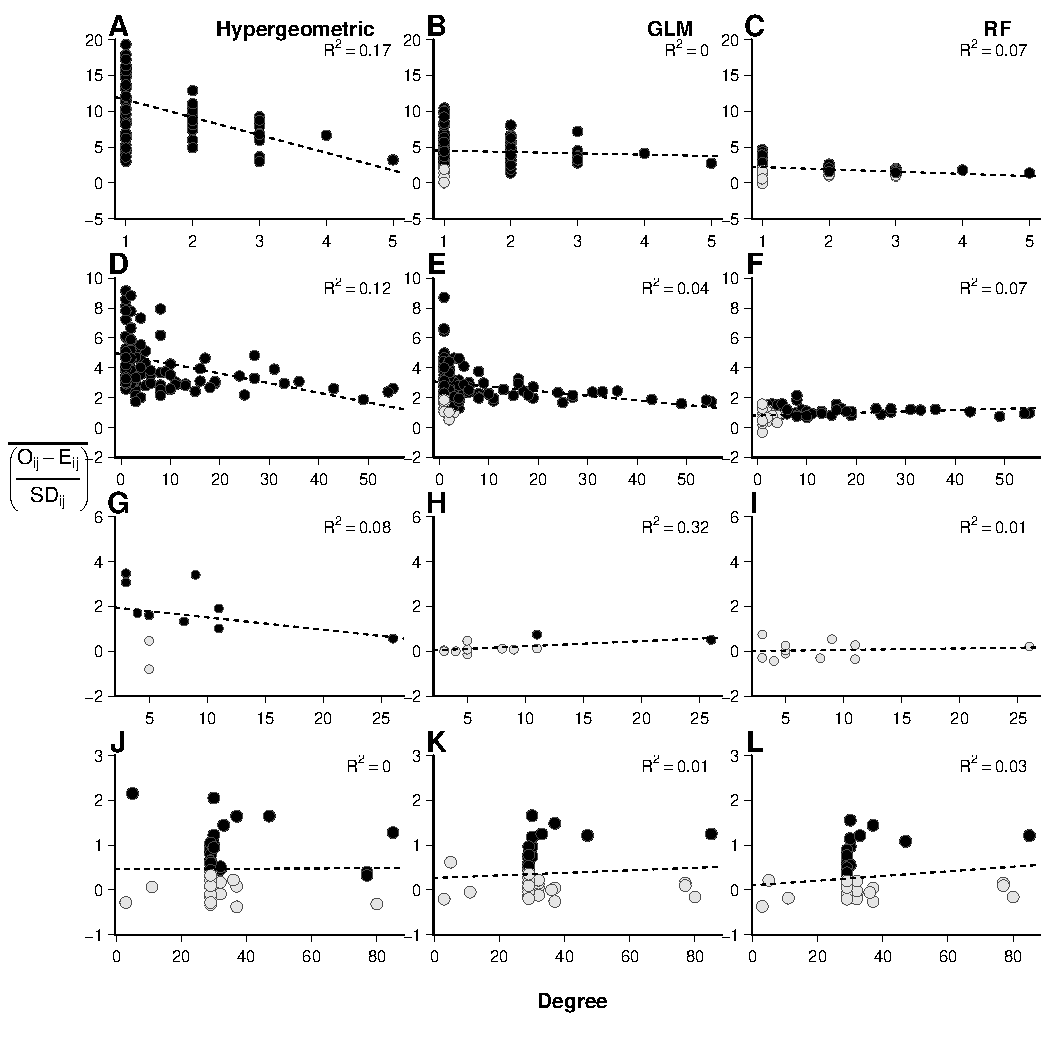
\includegraphics{chapitre3/figS7.pdf}
\caption{\textbf{The degree of species partially explains the decrease
of the co-occurrence strength} For the herbivores (A-C) and the
parasitoids in the willow leafs network datasets (D-F), the hummingbirds
in the Caribbean hummingbirds datasets (G-I) and all species in the
pitcher plants network that consume other species (J-L) the mean Z-score
is plotted against the degree of the species. Black symbols are mean
Z-scores significantly different from 0 (see SI Text). In each panel,
the dotted line represents the linear regression \(y~ax+b\) for which
the \(R^2\) is provided.\label{fig:degree}}
\end{figure}

\newpage

\begin{figure}[htbp]
\centering
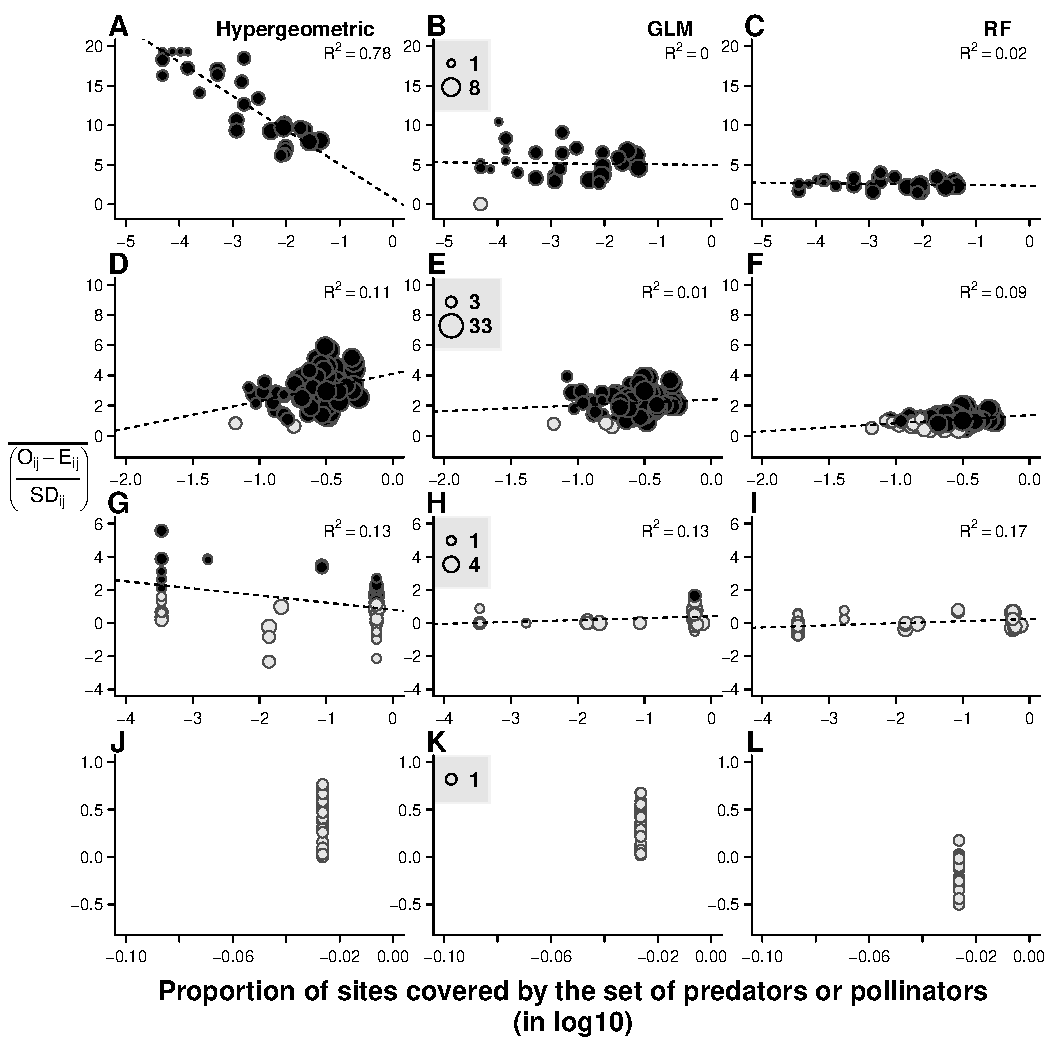
\includegraphics{chapitre3/figS8.pdf}
\caption{*Reversed figure 4** This figures correspond to the figure 4 in
the main text but the Z-score are calculated for preys (host plants)
rather than for predators 9pollinators). Mean Z-score are computed for
willows (A-C) and herbivores (based on the herbivores-parasitoids only,
D-F) of the willows leafs network, the hosts plants in the Caribbean
hummingbirds datasets (G-I) and species that feed on the detritus in the
pitcher plants network (panels J-L). The x-axis is expressed as a log
proportion of the total number of sites included in the considered
dataset. Black symbols are mean Z-scores significantly different from 0
(see SI Text). In each panel, the dotted line represents the linear
regression \(y~ax+b\) for which the \(R^2\) is provided. The size of
circles reflects the degree of species for which the Z-score was
calculated, the relation size-degree for each row is given in the middle
panel.\label{fig:degocc2}}
\end{figure}

\newpage

\begin{figure}[htbp]
\centering
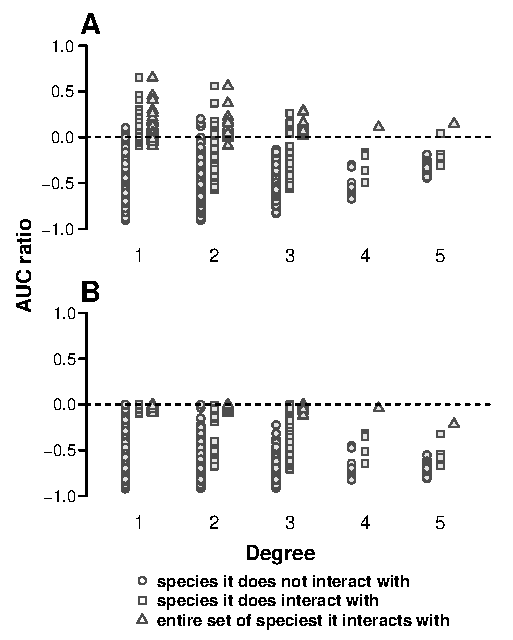
\includegraphics{chapitre3/figS9.pdf}
\caption{\textbf{Predicting herbivore distribution based on the
distribution of willows} For the herbivores in the willow leafs network
dataset, we compared the AUC obtained when using willow it does not
interact with (circles) a willow in interacts with (squares) and the set
of willow it interacts with (triangles) to AUC obtained for GLM (A) and
RF (B). Positive values indicated that species based model outperformed
the SDM model.\label{fig:ratauc}}
\end{figure}

\newpage

\newpage
